% !TEX TS-program = XeLaTeX
%!TEX encoding = UTF-8 Unicode
%==================================================
%      PREAMBOLO e DICHIARAZIONI INIZIALI
%==================================================
\documentclass[10pt,oneside,a4paper]{article}

\usepackage[utf8]{inputenc} 
\usepackage[italian]{babel}
\usepackage[T1]{fontenc}
\usepackage{siunitx} %Inserisce automaticamente i dati con le unità  di misura correttamente formattate del SI (utilizzo: \SI{0.82}{m^2}, in generale \SI{misura con il punto decimale}{unità  di misura})
\sisetup{output-decimal-marker = {.}, separate-uncertainty = true, input-uncertainty-signs = \pm, detect-weight=true, detect-family=true} %per usare SI con il punto decimale
\usepackage{listings} %Per citare codice informatico formattandolo correttamente
\usepackage{amsmath,amsthm,verbatim,amssymb,amsfonts,amscd,graphicx,mathtools}
\usepackage[makeroom]{cancel}
\newcommand{\abs}[1]{\left\lvert\,#1\,\right\rvert}
\usepackage{geometry}
\usepackage{epigraph}
\usepackage{booktabs}	%tabelle migliorate
\usepackage{tablefootnote}	%note a piè di pagina in tabella
\usepackage{threeparttable} %tabella con note a piè di tabella
\usepackage{caption}	%descrizione per figure
\usepackage{dblfnote}
\usepackage{supertabular}
\usepackage{longtable}
\captionsetup{tableposition=top,figureposition=bottom,font=small} %setup descrizione
\usepackage{float}
\usepackage{esvect} %vettori
\usepackage{longtable} %tabelle lunghe
\usepackage[dvipsnames]{xcolor}
\definecolor{sepia}{HTML}{80002A}
\usepackage[colorlinks=true, citecolor=black, linkcolor=sepia, urlcolor=black]{hyperref}
\usepackage{mathrsfs}
\usepackage{circuitikz}
\tikzset{
  font={\fontsize{7pt}{12}\selectfont}}
\ctikzset{bipoles/resistor/height=0.2}
\ctikzset{bipoles/resistor/width=0.4}
\ctikzset{bipoles/diode/height=0.3}
\ctikzset{bipoles/diode/width=0.3}
\ctikzset{tripoles/american nand port/height=0.7}
\ctikzset{tripoles/american nand port/width=0.8}
\usepackage{enumitem} %Liste senza spazi verticali
\setlist{noitemsep}
\usepackage{amsmath}
\usepackage{hyperref}
%\usepackage{pst-optexp} %Diagrammi ottici
\usepackage{physics} %Ambienti utili
\usepackage{upgreek} %Per avere lettere greche non corsive, ex. \upbeta


\interfootnotelinepenalty=10000


\usepackage{multicol}
\newenvironment{Figure}
  {\par\medskip\noindent\minipage{\linewidth}}
  {\endminipage\par\medskip}

%\newcommand{\var}{\operatorname{var}}
%\newcommand{\cov}{\operatorname{cov}}


\usepackage{listings} %Per inserire codice
\lstdefinestyle{CStyle}{
    backgroundcolor=\color{backgroundColour},   
    commentstyle=\color{mGreen},
    keywordstyle=\color{magenta},
    numberstyle=\tiny\color{mGray},
    stringstyle=\color{mPurple},
    basicstyle=\footnotesize\ttfamily,
    breakatwhitespace=false,         
    breaklines=true,                 
    captionpos=b,                    
    keepspaces=true,                 
    numbers=left,                    
    numbersep=5pt,                  
    showspaces=false,                
    showstringspaces=false,
    showtabs=false,                  
    tabsize=2,
    language=C
}

\definecolor{color1}{RGB}{90,0,0} % Color of the article title and sections
\definecolor{color2}{RGB}{0,20,50} % Color of the boxes behind the abstract and headings
\definecolor{mGreen}{rgb}{0,0.6,0}
\definecolor{mGray}{rgb}{0.5,0.5,0.5}
\definecolor{mPurple}{rgb}{0.58,0,0.82}
\definecolor{backgroundColour}{rgb}{0.95,0.95,0.92}


%==================================================
%                  PRIMA PAGINA
%==================================================

\title{\textsc{\textbf{Esperienza 5}: Studio della Polarizzazione mediante lamine di ritardo}}
\author{\small{G. Galbato Muscio} \and \small{F. Ghimenti} \and \small{L. Gravina} \and \small{L. Graziotto}}
\date{30 Maggio 2019}

\begin{document}
	\begin{figure}
		\centering
		
\includegraphics[scale=0.5, trim={2.8cm 8.9cm 0 9cm}, clip]{logo.png}
	\end{figure}
	\maketitle
	\begin{center} 
		\fbox{{\fontsize{12pt}{8mm}\textsc{Gruppo D1-1}}} \\
	\end{center}
\hrule
\vfill
\renewcommand{\abstractname}{Abstract}
\begin{abstract}
Si studia il funzionamento delle lamine di ritardo $\lambda / 2$ e $\lambda / 4$. Dopo averne determinato l'asse ottico, le si utilizza per realizzare un polarimetro. Mediante il polarimetro si misura quindi la polarizzazione della luce emessa dal laser He-Ne, sia direttamente, sia facendola passare per un beam-splitter polarizzatore o per un filtro polaroid.
\end{abstract}
\vfill
\tableofcontents %Indice
\newpage


\pagebreak


\begin{multicols}{2}
%==================================================
%             APPARATO STRUMENTALE
%==================================================
\section{Apparato strumentale}

Si utilizza un laser He-Ne di lunghezza d'onda, dichiarata dal costruttore, $\lambda = \SI{632.8}{nm}$, montato su tavolo ottico. 

In serie al laser è posta un'iride, allo scopo di evitare l'ingresso nel laser dei fasci di ritorno, che ne perturberebbero il comportamento. Due specchi orientati a \SI{45}{\degree} portano il fascio ad incidere su un primo beam-splitter polarizzatore, seguito dalle due lamine di ritardo $\lambda / 2$ e $\lambda / 4$ e dal secondo beam-splitter polarizzatore. Successivamente, è posto il fotodiodo, utilizzato per misurare l'intensità del fascio.

La configurazione utilizzata è illustrata in Figura~\ref{fig:diagram}.

\begin{Figure}
	\begin{center}
	\hbox{\hspace{-0.8cm}
	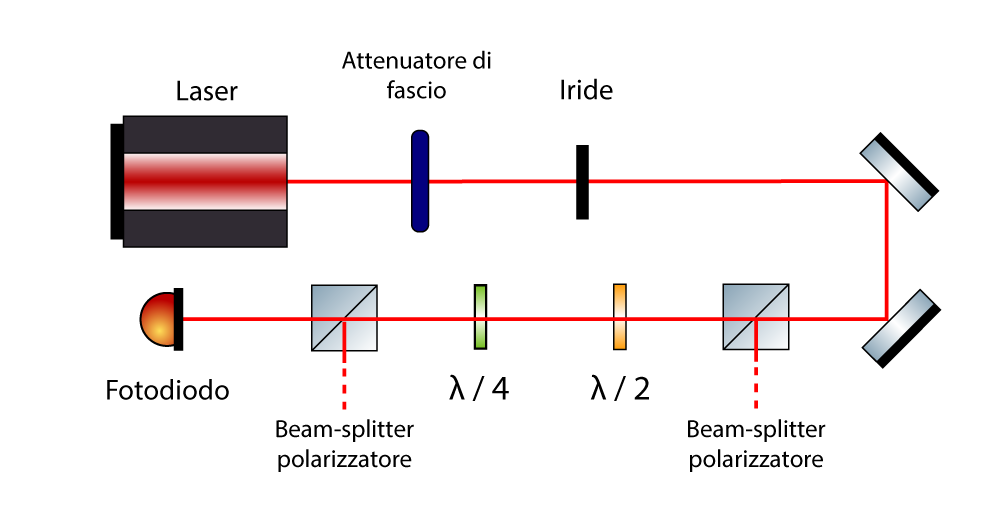
\includegraphics[width=1.1\linewidth]{diagram.png}}
	\captionof{figure}{Configurazione utilizzata.}
	\label{fig:diagram}
	\end{center}
\end{Figure}

Il segnale in uscita dal fotodiodo è inviato al multimetro \texttt{METEX M-4650}. Le misure di intensità luminosa vengono riportate come differenza di potenziale misurata ai capi del fotodiodo, pertanto è da intendere la presenza di un fattore di proporzionalità non noto.

%==================================================
%             TARATURA DEL POLARIMETRO
%==================================================
\section{Taratura del polarimetro}\label{sec:taratura}
In questa sezione si rimuove la lamina $\lambda / 4$. Si utilizza il primo beam splitter polarizzatore per ottenere una luce polarizzata orizzontalmente (linearmente, in un piano parallelo al piano del tavolo ottico), questa viene fatta passare attraverso una lamina di ritardo $\lambda/2$ montata su una ghiera graduata che permette di controllarne la rotazione; il fascio in uscita dalla lamina viene fatto passare nel secondo beam splitter che ne seleziona la sola componente orizzontale, infine l'intensità di questo fascio viene misurata con il fotodiodo. 

Si vuole trovare l'angolo $\theta_0$ della ghiera che corrisponde ad una situazione in cui l'asse principale della $\lambda/2$ è orizzontale.

In Figura \ref{fig:taratura_lambda2} è riportato l'andamento dell'intensità misurata al variare dell'angolo di rotazione della $\lambda/2$, mentre le misure sono riportate in Tabella \ref{tab:taratura_lambda2}, in Appendice. Ai punti sperimentali è sovrapposto un fit dell'andamento teorico dato da
\begin{equation}
	I(\theta) = I_0 \cos^2\big( 2(\theta- \theta_0)\big)
\end{equation}
dove i parametri che meglio descrivono le misure sono $I_0 = \SI{4.48 \pm 0.05}{V}$ e ${\theta_0 = \SI{0.680\pm0.005}{rad}}$.
\begin{Figure}
	\begin{center}
	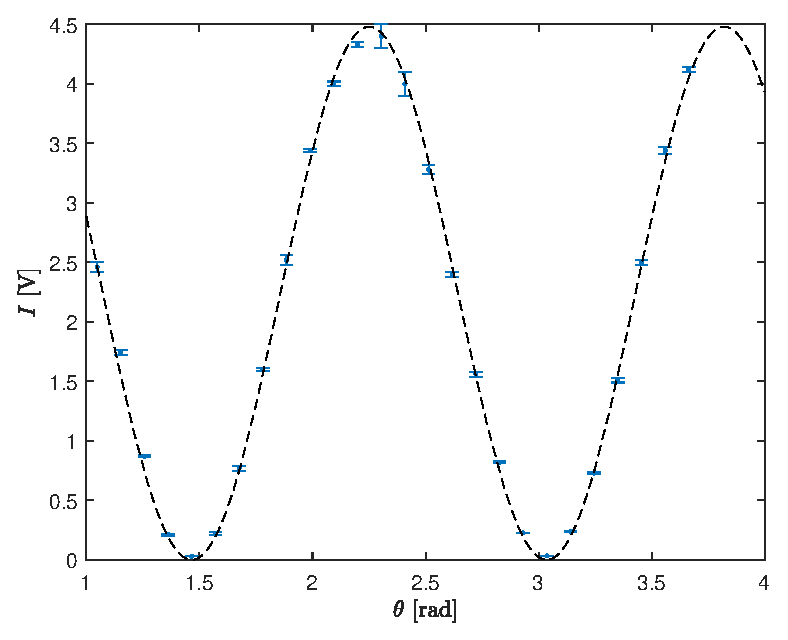
\includegraphics[width=0.9\linewidth]{taratura_lambda2.eps}
	\captionof{figure}{Andamento della tensione misurata dal fotodiodo al variare dell'angolo di rotazione della lamina $\lambda/2$, ai dati è sovrapposto il fit del modello teorico}
	\label{fig:taratura_lambda2}
	\end{center}
\end{Figure}

Valutato l'angolo $\theta_0$ corrispondente all'asse principale della $\lambda/2$, si valuta lo stesso angolo $\xi_0$ per la $\lambda/4$: quest'ultima viene montata tra il primo beam splitter e la $\lambda/2$, come da Figura~\ref{fig:diagram}. Avendo posizionato la seconda lamina di ritardo nella configurazione per cui l'asse è orizzontale (ossia all'angolo $\theta_0$ misurato precedentemente), si ruota la ghiera della $\lambda/4$ e si ottengono le misure riportate in Tabella \ref{tab:taratura_lambda4}, in Appendice, e in Figura \ref{fig:taratura_lambda4}; in quest'ultima è anche riportato il fit del modello teorico dato da
\begin{equation}
	I(\xi) = \frac{\tilde{I}_0}{2}\Big( 1- \cos^2\big(2(\xi-\xi_0)\big)\Big)
\end{equation}
dove i parametri del fit che meglio descrivono le misure sono $\tilde{I}_0 = \SI{7.6\pm0.1}{V}$ e $\xi_0 = \SI{0.19\pm0.02}{rad}$.
\begin{Figure}
	\begin{center}
	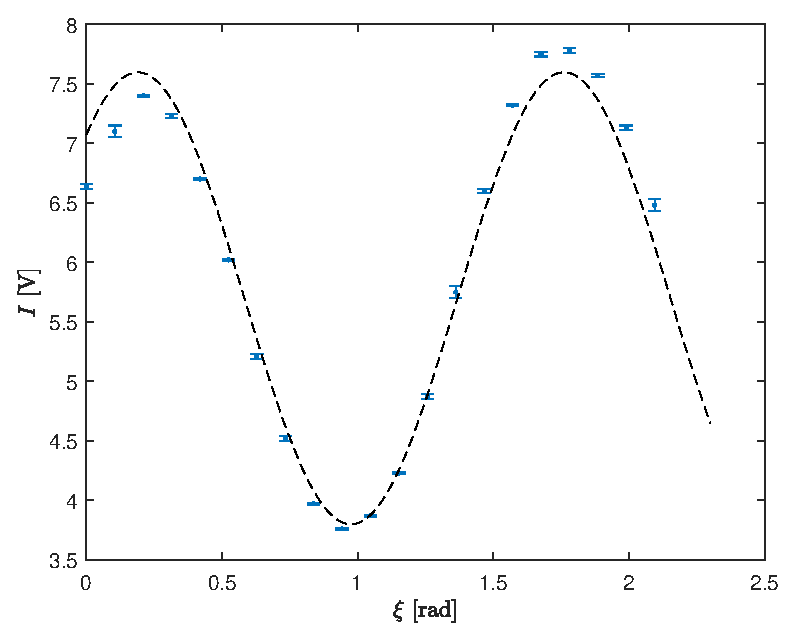
\includegraphics[width=0.9\linewidth]{taratura_lambda4.eps}
	\captionof{figure}{Andamento della tensione misurata dal fotodiodo al variare dell'angolo di rotazione della lamina $\lambda/4$, ai dati è sovrapposto il fit del modello teorico}
	\label{fig:taratura_lambda4}
	\end{center}
\end{Figure}
Il motivo per cui si è scritto $\tilde{I}_0$ invece di $I_0$ è che nel caso ideale queste due quantità dovrebbero coincidere, ma nel corso dell'esperienza tra la taratura di $\lambda/2$ e quella di $\lambda/4$ sono state effettuate delle importanti operazioni di allineamento del sistema, che hanno comportato anche una modifica dell'intensità massima del fascio.

Infine, si osserva che il fit relativo alla taratura della $\lambda/4$ si discosta maggiormente dai punti sperimentali rispetto a quello della $\lambda/2$; in particolare, si confronta un coefficiente $R^2 = 0.998$ per la $\lambda/2$ con $R^2 = 0.976$ per la $\lambda/4$. Si suppone che questo sia dovuto al fatto che la $\lambda/4$ è molto più sensibile a imprecisioni nell'allineamento rispetto alla $\lambda/2$.


%==================================================
%            CONTROLLO SULL'ALLINEAMENTO
%==================================================
\section{Controllo di funzionamento del polarimetro}

Si verifica il corretto allineamento delle lamine di ritardo nel modo seguente: la lamina $\lambda/4$ viene tenuta fissa ad un angolo pari a $\xi_0 + 45\SI{}{\degree}$ mentre si varia l'angolo $\theta$ della lamina $\lambda/2$. Si misura l'intensità della luce all'uscita del secondo beam-splitter polarizzatore. I risultati sono riportati in Figura~\ref{fig:align} e nella Tabella~\ref{tab:align}, in Appendice. In questa configurazione si prevede che l'intensità misurata in funzione di $\theta$ sia costante; si realizza dunque un fit lineare dei dati sperimentali e si ottiene come valore del coefficiente angolare $m = \SI{4 \pm 2 e-4}{V / \text{grado}}$, compatibile con zero entro due deviazioni standard. Si osserva tuttavia un andamento sinusoidale, di ampiezza ridotta (al massimo \SI{0.5}{V}), che si ritiene sia dovuto a imperfezioni nelle lamine, che attenuano l'intensità della luce in maniera non omogenea rispetto alla direzione di polarizzazione. 

\begin{Figure}
	\begin{center}
	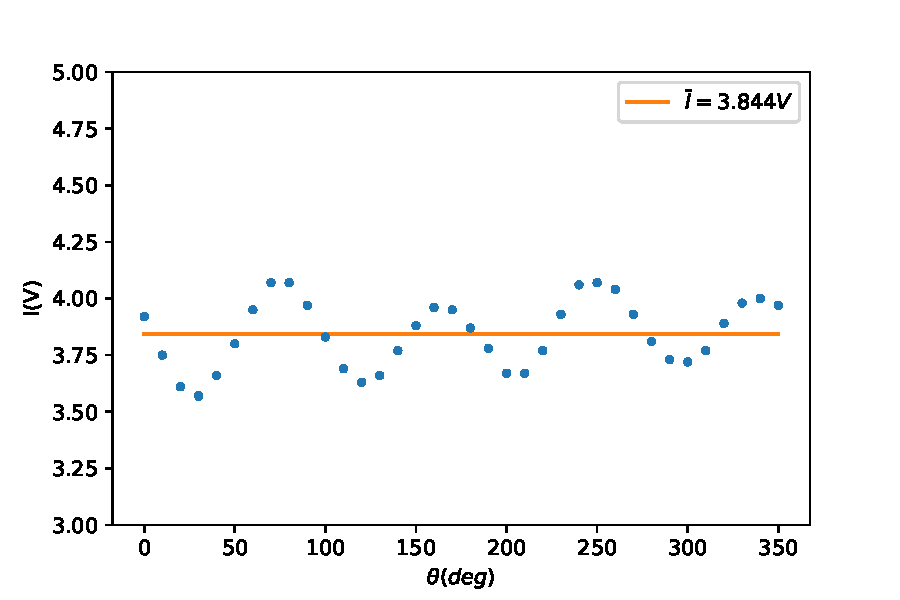
\includegraphics[width=0.9\linewidth]{align.pdf}
	\captionof{figure}{Intensità misurata con $\lambda / 4$ a $\xi + 45 \SI{}{\degree}$ e al variare di $\theta$ della $\lambda / 2$}
	\label{fig:align}
	\end{center}
\end{Figure}


%==================================================
%            MISURA DELLA POLARIZZAZIONE
%==================================================
\section{Misura della polarizzazione della luce emessa dal laser He-Ne}
In questa sezione si utilizza l'intera configurazione di Figura~\ref{fig:diagram}, tenuto conto che gli assi ottici delle lamine di ritardo $\lambda / 2$ e $\lambda / 4$ sono quelli misurati nella Sezione~\ref{sec:taratura}, ovvero
\[
\begin{aligned}
\theta_0 &= \SI{0.680\pm0.005}{rad} = \SI{39.0 \pm 0.3}{\degree} \\
\xi_0 &= \SI{0.19\pm0.02}{rad} = \SI{11.0 \pm 1.1}{\degree};
\end{aligned}
\]
si ricorda che l'incertezza sulla ghiera goniometrica che permette la rotazione delle lamine è di $1$ grado. Gli angoli di orientazione delle lamine necessari a misurare i diversi parametri di Stokes sono riferiti, nel seguito, alla posizione angolare dell'asse ottico.

I parametri di Stokes normalizzati sono
\[
\begin{aligned}
s_1 &= \frac{I_1 - I_1'}{I_1 + I_1'} \\
s_2 &= \frac{I_2 - I_2'}{I_2 + I_2'} \\
s_3 &= \frac{I_3 - I_3'}{I_3 + I_3'};
\end{aligned}
\]
essi sono compresi tra $0$ e $1$, e si riferiscono, rispettivamente, alla polarizzazione lineare orizzontale e verticale, lineare a \SI{45}{\degree} e \SI{-45}{\degree} e circolare left e right. La misura di $I_i$ è compiuta ruotando le lamine di ritardo agli angoli riportati in Tabella~\ref{tab:misuraStokes}, in Appendice.

Si osserva che con la normalizzazione sopra riportata si possono trascurare effetti di instabilità del laser o di deriva della intensità del fondo, nonché delle perdite per assorbimento per i vari componenti.

\subsection{Misura dei parametri di Stokes per luce uscente dal beam splitter}
Si misura la polarizzazione della luce emessa dal laser He-Ne dopo che essa ha attraversato il primo beam-splitter polarizzatore, lasciando invariata dunque la configurazione del sistema. Si riportano in Tabella~\ref{tab:stokesBS}, in Appendice, i dati sperimentali; si ottengono per i parametri di Stokes i seguenti valori:
\[
\begin{aligned}
s_1 &= \SI{0.974 \pm 0.003}{} \\
s_2 &= \SI{0.072 \pm 0.003}{}\\
s_3 &= \SI{0.017 \pm 0.003}{};\\
\end{aligned}
\]
si ha il grado di polarizzazione $s^2 = (s_1^2+s_2^2+s_3^2)^{1/2} = \SI{0.977 \pm 0.003}{}$, prossimo a $1$, come ci si aspetterebbe per luce completamente polarizzata. Si osserva che il parametro relativo alla polarizzazione lineare orizzontale risulta di un ordine di grandezza superiore a $s_2$ e $s_3$, in accordo con l'assunzione iniziale che il beam splitter polarizzatore lasci passare unicamente la polarizzazione orizzontale. La discrepanza rispetto al valore di $1$ per $s_1$ e di $0$ per gli altri parametri è da attribuire ad effetti di assorbimento, al non perfetto allineamento dei fasci e alla non completa planarità delle superfici delle lamine.

\subsection{Misura dei parametri di Stokes per luce emessa dal laser}
Si rimuove il primo beam splitter polarizzatore, e lo si pone dopo il secondo polarizzatore, per migliorare la selezione della polarizzazione in uscita dal polarimetro. In questo modo, sul polarimetro (ovvero sulla prima lamina di ritardo $\lambda / 2$) incide direttamente la luce emessa dal laser He-Ne, di cui si può pertanto dare una stima della polarizzazione. Si riportano in Tabella~\ref{tab:stokesHeNe}, in Appendice, i dati sperimentali; i parametri di Stokes sono i seguenti:
\[
\begin{aligned}
s_1 &= \SI{0.65 \pm 0.01}{} \\
s_2 &= \SI{-0.755 \pm 0.001}{}\\
s_3 &= \SI{0.037 \pm 0.009}{};\\
\end{aligned}
\]
si ha il grado di polarizzazione $s^2 = (s_1^2+s_2^2+s_3^2)^{1/2} = \SI{0.998 \pm 0.008}{}$, compatibile con $1$, valore che indica la completa polarizzazione. Pertanto si inferisce che la luce del laser He-Ne sia totalmente polarizzata e, dall'osservazione del fatto che il parametro di Stokes relativo alla polarizzazione circolare $s_3$ sia di almeno un ordine di grandezza inferiore agli altri due, relativi alla polarizzazione lineare, si può escludere che vi sia una consistente componente di polarizzazione circolare nella luce emessa.

Si può fornire una rappresentazione grafica del campo elettrico della luce emessa dal laser He-Ne, definendo i valori sul piano ortogonale al banco ottico nel modo seguente (tenendo conto che si osserva solo il rapporto tra le due componenti in $x$ e $y$, in quanto non è noto il fattore di normalizzazione):
\[
\begin{aligned}
E_{0x} &= s_1 + \sqrt{s_1^2+s_2^2+s_3^2} \\
E_{0y} &= -s_1 + \sqrt{s_1^2+s_2^2+s_3^2},
\end{aligned}
\]
e lo sfasamento tra le due componenti è dato da $\delta = \arctan(s_3/s_2)$. Con un plot polare si ottiene il grafico di Figura~\ref{fig:Efield}, ove si osserva che la luce è polarizzata ellitticamente, ma essendo l'ellisse molto eccentrica essa si avvicina alla polarizzazione lineare. 

\begin{Figure}
	\begin{center}
	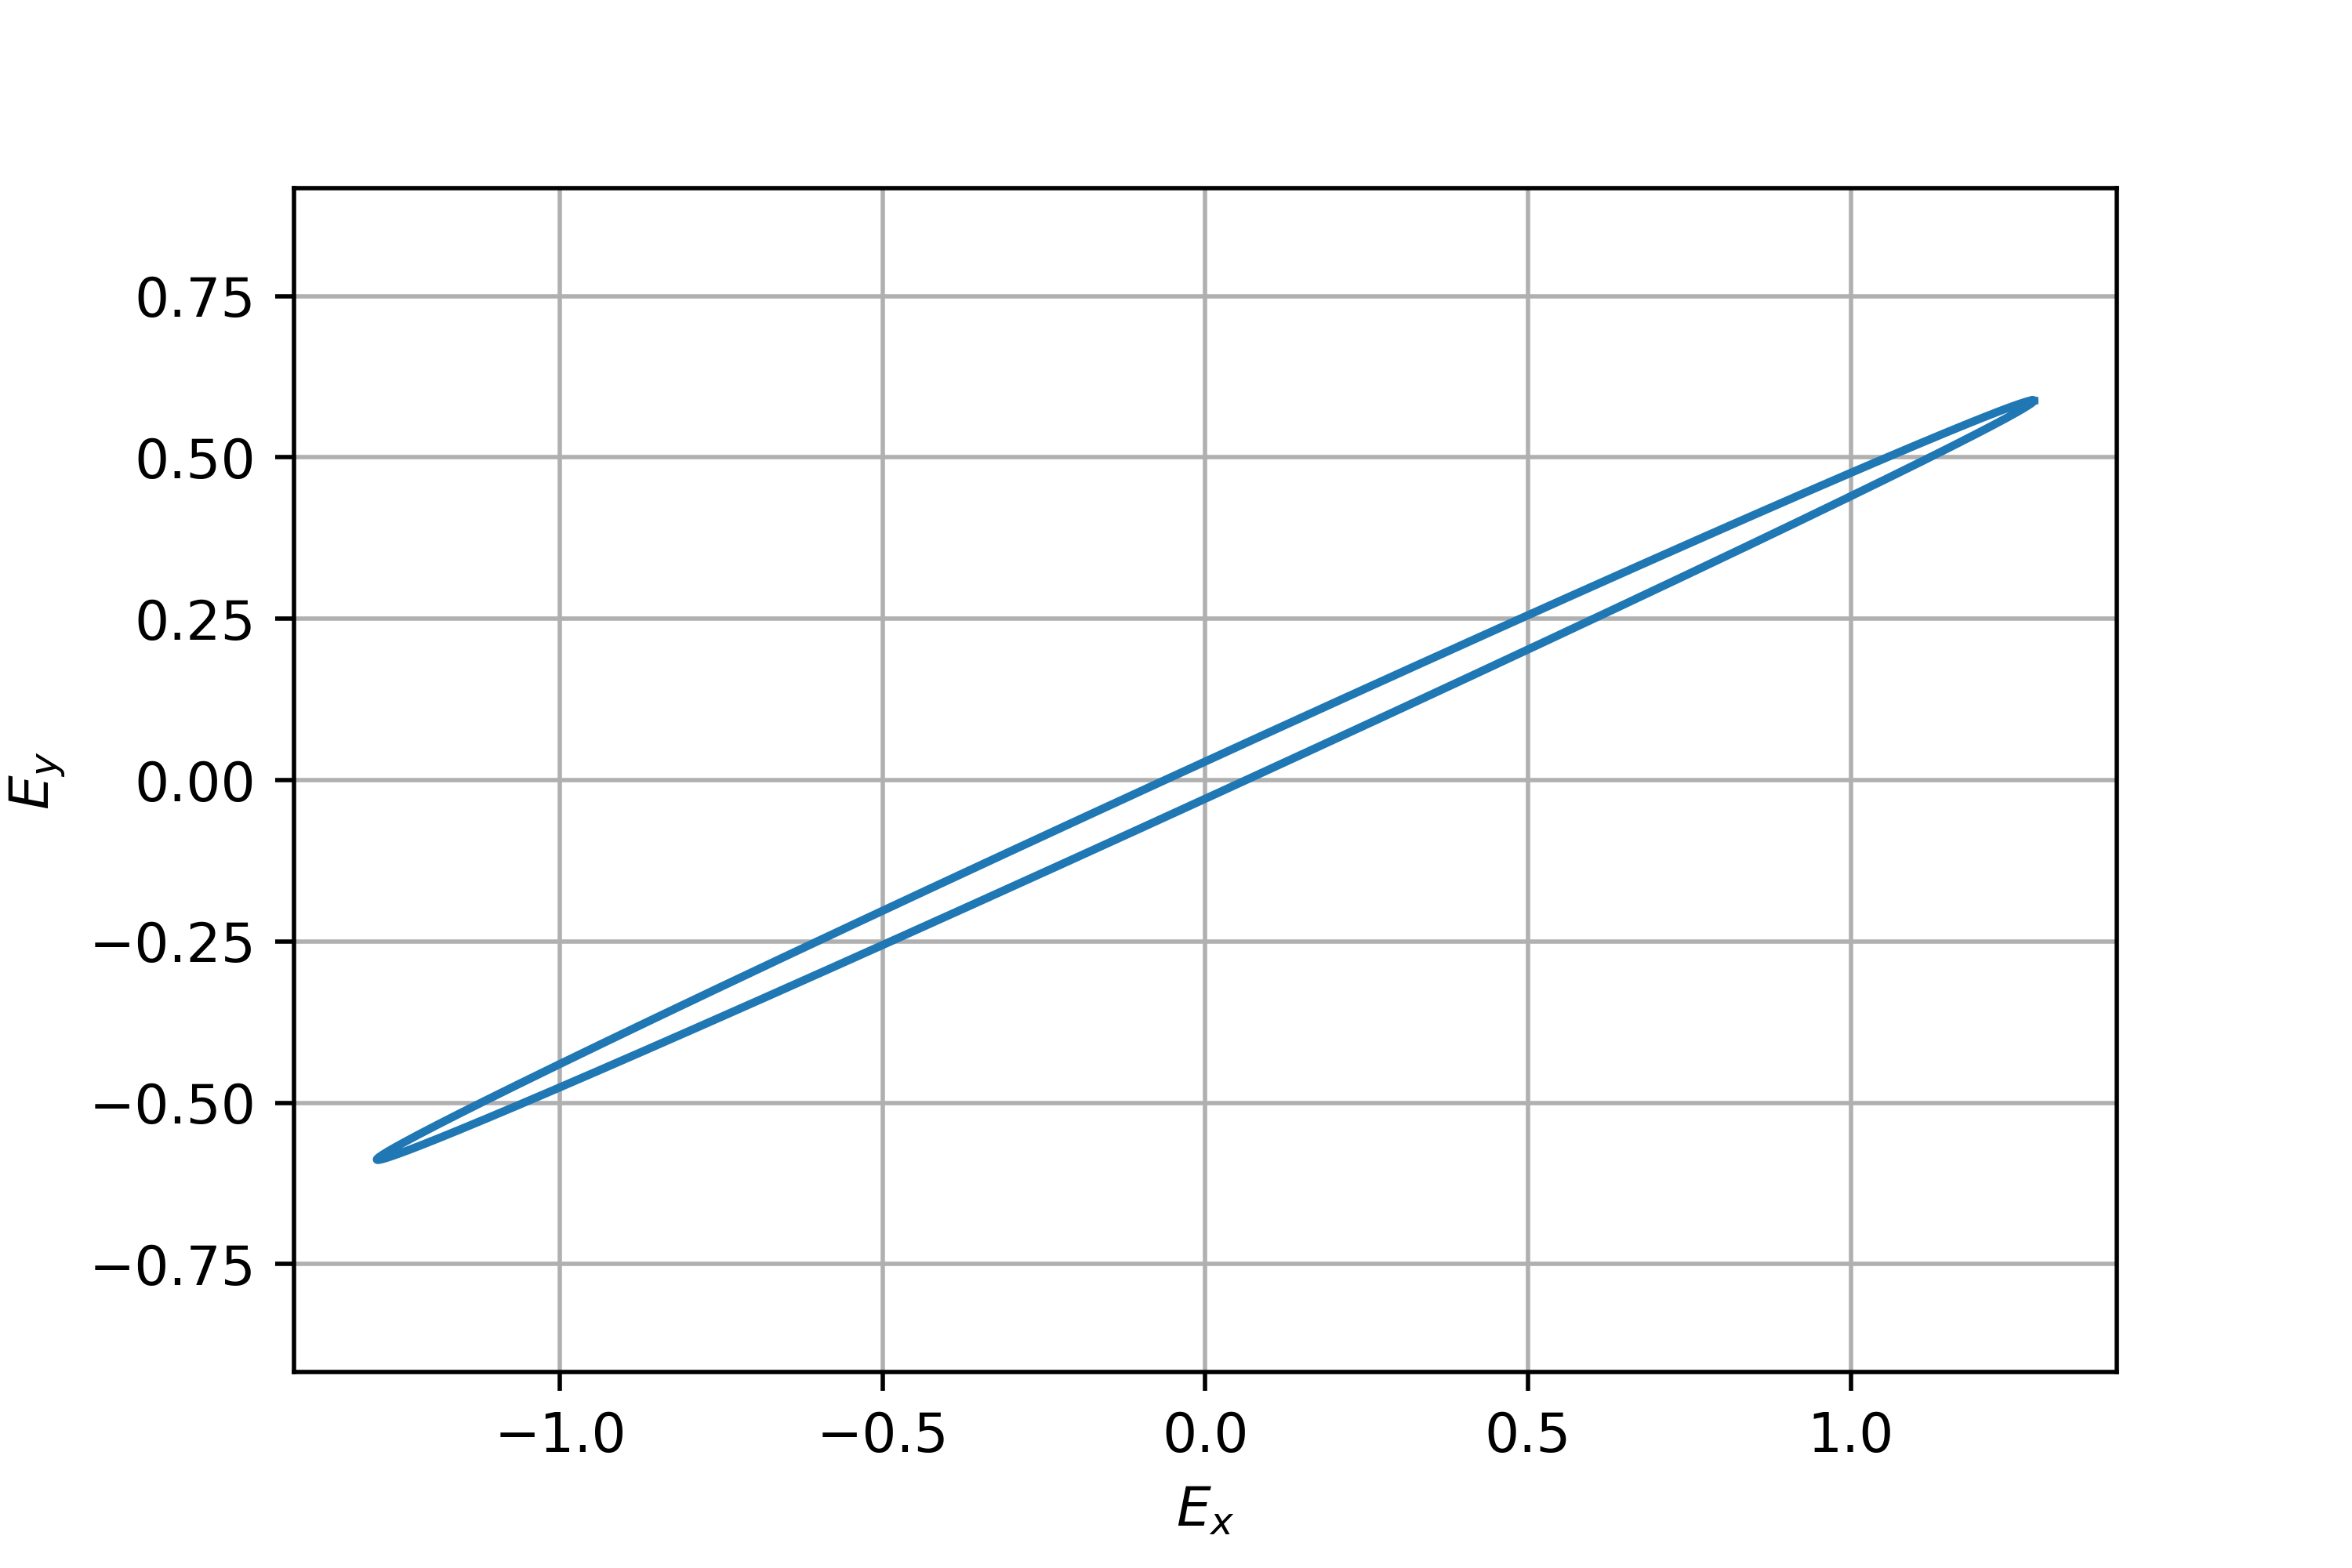
\includegraphics[width=\linewidth]{Efield.png}
	\captionof{figure}{Rappresentazione grafica del campo elettrico della luce uscente dal laser He-Ne}
	\label{fig:Efield}
	\end{center}
\end{Figure}

\subsection{Misura dei parametri di Stokes per luce polarizzata linearmente con un polaroid}
Si mantiene inalterato il setup sperimentale aggiungendo un filtro polarizzatore prima della $\lambda/4$. Ruotando il polarizzatore si varia la polarizzazione del fascio, mappando i punti sulla sfera di Poincaré. Gli stati con polarizzazione pura si trovano sulla superficie della sfera, in quanto $s^2 =1$, mentre gli stati misti si trovano all’interno, avendo $s^2<1$. I dati sperimentali sono riportati in Tabella~\ref{tab:ultima}. Si riportano in Figura~\ref{fig:piano} e~\ref{fig:spazio} i grafici nel piano e nello spazio dei coefficienti di Stokes. 

\begin{Figure}
	\begin{center}
	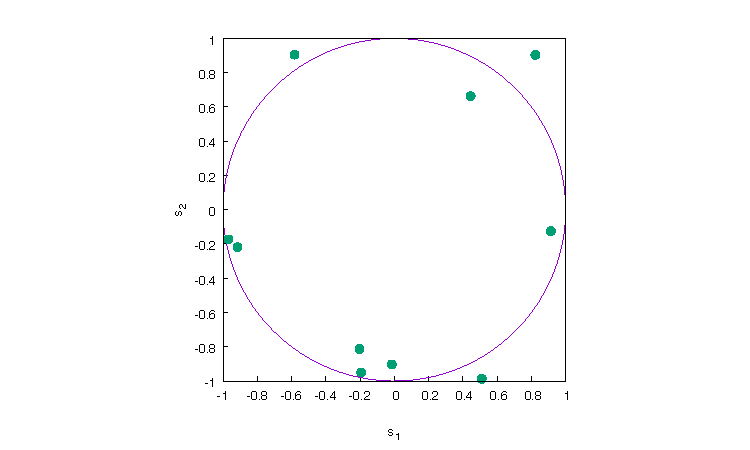
\includegraphics[width=\linewidth]{piano}
	\captionof{figure}{Rappresentazione grafica del cerchio di Poincaré nel sistema di coordinate di Stokes}
	\label{fig:piano}
	\end{center}
\end{Figure}
\begin{Figure}
	\begin{center}
	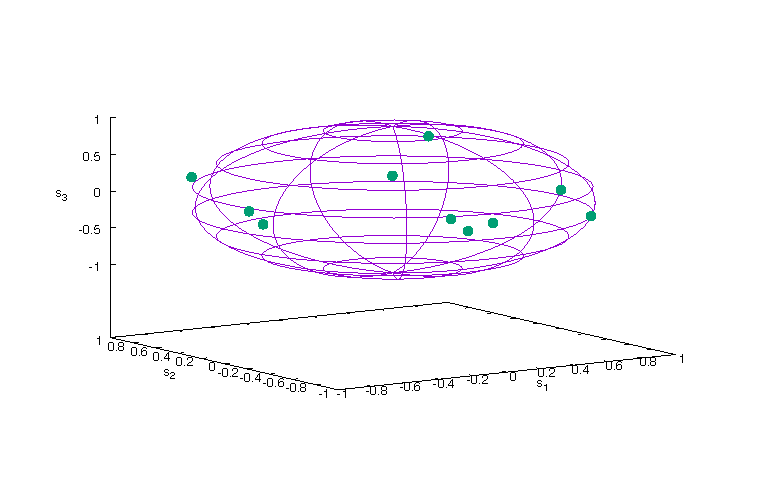
\includegraphics[width=\linewidth]{spazio}
	\captionof{figure}{Rappresentazione grafica della sfera di Poincaré nel sistema di coordinate di Stokes}
	\label{fig:spazio}
	\end{center}
\end{Figure}

Si osserva che i punti sperimentali sono per la maggior parte all'interno della sfera di Poincaré; i punti esterni con $s^2>1$ non hanno senso fisico e sono da imputare ad imperfezioni nel polaroid o ad un non corretto allineamento dei fasci.



%==================================================
%             CONCLUSIONI
%==================================================
\section{Conclusioni}
Mediante il polarimetro realizzato con le lamine di ritardo $\lambda / 4$ e $\lambda / 2$ si è misurata la polarizzazione del laser He-Ne, che risulta essere prevalentemente lineare, con ridotta componente polarizzata circolarmente. Nel realizzare il polarimetro si è rivelato cruciale il corretto allineamento di tutti i fasci, in particolare dell'interfaccia della lamina $\lambda / 4$, che risulta essere più sensibile a lievi deviazioni dalla condizione di ortogonalità. Il controllo sul funzionamento del polarimetro ne ha confermato l'accuratezza, comunque affetta da imperfezioni dovute alla non completa planarità delle superfici e alle eventuali impurità presenti sulle stesse.

La mappatura dei punti sulla sfera di Poincaré per stati della luce a polarizzazione lineare devia in alcuni casi dalla previsione teorica, e si ritiene che questo sia dovuto ad un non corretto allineamento del polarizzatore stesso, o all'usura delle superfici.

\end{multicols}


\newpage
\section{Appendice}

\begin{minipage}[t]{0.3\linewidth}
\begin{center}
\captionof{table}{Punti sperimentali per la taratura della lamina $\lambda / 2$}
\label{tab:taratura_lambda2}
\begin{tabular}{c|c|c}
\toprule
     $\theta$ [\SI{}{\degree}] &    $I$ [\SI{}{V}] &   $\sigma_I$ [\SI{}{V}]\\
     $\pm 0.1$ & & \\
\midrule
  60.0 &  2.46 &  0.04 \\
  66.0 &  1.74 &  0.02 \\
  72.0 &  0.87 &  0.01 \\
  78.0 &  0.21 &  0.01 \\
  84.0 &  0.030 &  0.001 \\
  90.0 &  0.22 &  0.01 \\
  96.0 &  0.77 &  0.02 \\
 102.0 &  1.60 &  0.01 \\
 108.0 &  2.52 &  0.04 \\
 114.0 &  3.44 &  0.01 \\
 120.0 &  4.00 &  0.02 \\
 126.0 &  4.33 &  0.02 \\
 132.0 &  4.40 &  0.10 \\
 138.0 &  4.00 &  0.10 \\
 144.0 &  3.28 &  0.04 \\
 150.0 &  2.40 &  0.02 \\
 156.0 &  1.56 &  0.02 \\
 162.0 &  0.82 &  0.01 \\
 168.0 &  0.226 &  0.002 \\
 174.0 &  0.033 &  0.001 \\
 180.0 &  0.239 &  0.002 \\
 186.0 &  0.73 &  0.01 \\
 192.0 &  1.51 &  0.02 \\
 198.0 &  2.50 &  0.02 \\
 204.0 &  3.44 &  0.03 \\
 210.0 &  4.12 &  0.02 \\
\bottomrule
\end{tabular}
\end{center}
\end{minipage}
\hspace{1em}
\begin{minipage}[t]{0.3\linewidth}
\begin{center}
\captionof{table}{Punti sperimentali per la taratura della lamina $\lambda / 4$}
\label{tab:taratura_lambda4}
\begin{tabular}{c|c|c}
\toprule
     $\xi$ [\SI{}{\degree}] &    $I$ [\SI{}{V}] &   $\sigma_I$ [\SI{}{V}]\\
     $\pm 0.1$ & & \\
\midrule
   0.0 &  6.64 &  0.02 \\
   6.0 &  7.10 &  0.05 \\
  12.0 &  7.40 &  0.01 \\
  18.0 &  7.23 &  0.02 \\
  24.0 &  6.70 &  0.01 \\
  30.0 &  6.02 &  0.01 \\
  36.0 &  5.21 &  0.02 \\
  42.0 &  4.52 &  0.02 \\
  48.0 &  3.97 &  0.01 \\
  54.0 &  3.76 &  0.01 \\
  60.0 &  3.87 &  0.01 \\
  66.0 &  4.23 &  0.01 \\
  72.0 &  4.87 &  0.02 \\
  78.0 &  5.75 &  0.05 \\
  84.0 &  6.60 &  0.02 \\
  90.0 &  7.32 &  0.01 \\
  96.0 &  7.75 &  0.02 \\
 102.0 &  7.78 &  0.02 \\
 108.0 &  7.57 &  0.01 \\
 114.0 &  7.13 &  0.02 \\
 120.0 &  6.48 &  0.05 \\
\bottomrule
\end{tabular}
\end{center}
\end{minipage}
\hspace{1em}
\begin{minipage}[t]{0.3\linewidth}
\begin{center}
\captionof{table}{Punti sperimentali per la verifica dell'allineamento delle due lamine}
\label{tab:align}
\begin{tabular}{c|c|c}
\toprule
$\theta$[\SI{}{\degree}] &  $I$ [\SI{}{V}] &  $\sigma_{I}$ [\SI{}{V}] \\
     $\pm 0.1$ & & \\
\midrule
0.0 &    3.92 &            0.01 \\
10.0 &    3.75 &            0.01 \\
20.0 &    3.61 &            0.01 \\
30.0 &    3.57 &            0.02 \\
40.0 &    3.66 &            0.01 \\
50.0 &    3.800 &            0.005 \\
60.0 &    3.950 &            0.005 \\
70.0 &    4.07 &            0.01 \\
80.0 &    4.07 &            0.005 \\
90.0 &    3.97 &            0.01 \\
100.0 &    3.83 &            0.01 \\
110.0 &    3.690 &            0.005 \\
120.0 &    3.63 &            0.01 \\
130.0 &    3.66 &            0.01 \\
140.0 &    3.77 &            0.01 \\
150.0 &    3.880 &            0.005 \\
160.0 &    3.960 &            0.005 \\
170.0 &    3.95 &            0.001 \\
180.0 &    3.870 &            0.005 \\
190.0 &    3.780 &            0.005 \\
200.0 &    3.670 &            0.005 \\
210.0 &    3.67 &            0.01 \\
220.0 &    3.77 &            0.01 \\
230.0 &    3.930 &            0.005 \\
240.0 &    4.06 &            0.001 \\
250.0 &    4.070 &            0.005 \\
260.0 &    4.04 &            0.01 \\
270.0 &    3.93 &            0.01 \\
280.0 &    3.810 &            0.005 \\
290.0 &    3.73 &            0.01 \\
300.0 &    3.720 &            0.005 \\
310.0 &    3.77 &            0.01 \\
320.0 &    3.89 &            0.01 \\
330.0 &    3.980 &            0.005 \\
340.0 &    4.00 &            0.01 \\
350.0 &    3.97 &            0.01 \\
\bottomrule
\end{tabular}
\end{center}
\end{minipage}

\vspace{1cm}
\begin{minipage}[t]{.33\linewidth}
\begin{center}
\captionof{table}{Orientazione delle lamine per la misura dei parametri di Stokes}
\label{tab:misuraStokes}
\begin{tabular}{c|c|c}
 &  $\lambda / 4$: $\xi-\xi_0$ & $\lambda / 2$: $\theta-\theta_0$  \\
\hline
     $I_1$  &        \SI{0}{\degree} &         \SI{0}{\degree} \\
     $I_1'$  &       \SI{0}{\degree} &         \SI{45}{\degree} \\
     \hline 
     $I_2$  &        \SI{45}{\degree} &         \SI{22.5}{\degree} \\
     $I_2'$  &       \SI{45}{\degree} &         \SI{-22.5}{\degree} \\
     \hline 
     $I_3$  &        \SI{0}{\degree} &         \SI{22.5}{\degree} \\
     $I_3'$	&		 \SI{90}{\degree} &         \SI{22.5}{\degree} \\
\hline
\end{tabular}
\end{center}
\end{minipage}
\hspace{1em}
\begin{minipage}[t]{.33\linewidth}
\begin{center}
\captionof{table}{Punti sperimentali per la misura dei parametri di Stokes della luce uscente dal primo beam splitter polarizzatore}
\label{tab:stokesBS}
\begin{tabular}{c|c}
& Intensità [\SI{}{V}]  \\
\hline
     $I_1$  &        \SI{6.94 \pm 0.01}{} \\
     $I_1'$  &       \SI{0.090 \pm 0.001}{} \\
     \hline 
     $I_2$  &        \SI{4.04 \pm 0.01}{} \\
     $I_2'$  &       \SI{3.50 \pm 0.01}{} \\
     \hline 
     $I_3$  &        \SI{3.31 \pm 0.01}{} \\
     $I_3'$	&		 \SI{3.20 \pm 0.01}{} \\
\hline
\end{tabular}
\end{center}
\end{minipage}
\hspace{1em}
\begin{minipage}[t]{.33\linewidth}
\begin{center}
\captionof{table}{Punti sperimentali per la misura dei parametri di Stokes della luce uscente direttamente dal laser}
\label{tab:stokesHeNe}
\begin{tabular}{c|c}
& Intensità [\SI{}{V}]  \\
\hline
     $I_1$  &        \SI{7.95 \pm 0.05}{} \\
     $I_1'$  &       \SI{1.68 \pm 0.01}{} \\
     \hline 
     $I_2$  &        \SI{1.22 \pm 0.01}{} \\
     $I_2'$  &       \SI{8.74 \pm 0.04}{} \\
     \hline 
     $I_3$  &        \SI{4.20 \pm 0.05}{} \\
     $I_3'$	&		 \SI{3.90 \pm 0.02}{} \\
\hline
\end{tabular}
\end{center}
\end{minipage}
\newline

\vspace{2cm}

\begin{center}
\captionof{table}{Punti sperimentali per la misura dei parametri di Stokes della luce polarizzata con un polaroid}
\label{tab:ultima}
\begin{tabular}{c|c|c|c|c|c|c}
\toprule
$\theta$ [\SI{}{\degree}] & $I_1$ [\SI{}{V}] & $\sigma_{I_1}$ [\SI{}{V}] & $I_1'$ [\SI{}{V}] & $\sigma_{I_1'}$ [\SI{}{V}] & $I_2$ [\SI{}{V}] & $\sigma_{I_2}$ [\SI{}{V}]   \\
\midrule
  0  & 2.190 & 0.002 & 3.24 & 0.01 & 0.177 & 0.001 		\\		
  60 & 4.41 & 0.01 & 0.43 & 0.01 & 2.35 & 0.01 			\\		
 120 & 0.018 & 0.001 & 0.41 & 0.01 & 0.467 	& 0.001 	\\		
 180 & 2.560 & 0.005 & 2.64 & 0.01 	& 0.294 & 0.001 	\\		
 240 & 3.37 & 0.01 & 0.45 & 0.01 & 1.84 & 0.02 			\\		
 300 & 0.02 & 0.001 & 0.57 & 0.01 & 0.505 & 0.003 		\\		
  20 & 5.30 & 0.03 & 0.24 & 0.01 & 2.52 & 0.02 			\\		
  40 & 2.16 & 0.02 & 0.83 & 0.01 & 3.20 & 0.02 			\\		
  80 & 0.014 & 0.001 & 0.05 & 0.02 & 0.24 & 0.01 		\\		
 100 & 0.021 & 0.001 & 1.30 & 0.03 & 0.153 & 0.001 		\\		
 140 & 2.300 & 0.005 & 3.47 & 0.01 & 0.483 & 0.001 		\\		
 160 & 5.30 & 0.02 & 1.72 & 0.01 & 0.046 & 0.001 		\\		
 \bottomrule
\end{tabular}

\vspace*{0.4cm}
\centering
\begin{tabular}{c|c|c|c|c|c|c}
\toprule
$\theta$ [\SI{}{\degree}] & $I_2'$ [\SI{}{V}] & $\sigma_{I_2'}$ [\SI{}{V}] & $I_3$ [\SI{}{V}] & $\sigma_{I_3}$ [\SI{}{V}] & $I_3'$ [\SI{}{V}] & $\sigma_{I_3'}$ [\SI{}{V}] \\
\midrule
  0  & 6.90 & 0.01 & 2.998 & 0.007 & 3.29 & 0.01 \\
  60 & 0.119 & 0.001 & 0.70 & 0.01 & 0.342 & 0.001 \\
 120 & 0.729 & 0.003 & 1.43 & 0.01 & 1.55 & 0.01 \\
 180 & 5.76 & 0.01 & 2.45 & 0.01 & 2.42 & 0.01 \\
 240 & 0.069 & 0.001 & 0.445 & 0.001 & 0.195 & 0.002 \\
 300 & 1.054 & 0.005 & 1.553 & 0.004 & 1.69 & 0.01 \\
  20 & 3.24 & 0.01 & 2.49 & 0.01 & 2.70 & 0.01 \\
  40 & 0.65 & 0.01 & 1.652 & 0.004 & 1.71 & 0.01 \\
  80 & 0.012 & 0.001 & 0.027 & 0.001 & 0.021 & 0.001 \\
 100 & 0.217 & 0.001 & 0.432 & 0.001 & 0.330 & 0.002 \\
 140 & 4.68 & 0.02 & 2.584 & 0.003 & 2.24 & 0.01 \\
 160 & 7.02 & 0.01 & 3.24 & 0.01 & 3.22 & 0.01 \\
 \bottomrule
\end{tabular}
\end{center}



\end{document}
